\chapter{Analysis}
\label{chap:analysis}

Adjusting the fixed score for n-graph features having only a single occurrence (SO) in the reference had minimal impact on detection performance.
This was expected, as these are relatively rare.
For that reason, it is natural that features from probe actions either have none or several occurrences in the reference more often than only a single occurrence.
We observed that adjusting the fixed score for n-graphs missing in the reference had significant impact on the ANIA and ANGA ratings.


For example, when using the function seen in \Cref{fig:sig185}, we tested adjusting the fixed score for single and no occurrences (NO).
The results of these tests can be found in \Cref{tab:adjusting-SO-NO}.
The CA system becomes more strict as the SO and NO scores are increased, as this means that the trust levels are affected more negatively.
However, it has a larger impact on ANIA than ANGA.
Furthermore, we also tested the impact of lowering the SO score while keeping the NO score near maximum.
The result of this test can be seen in the last section of \Cref{tab:adjusting-SO-NO}.
Compared to the section above, it seems that the NO score has a much larger impact.
We can also see that the performance was negatively affected by using a low SO score, as 4 more imposters went undetected, and one user was moved from the -/+ category to the -/- category.
Therefore, it seems that having harsh punishments for n-graphs not present or with only a single occurrence in the reference leads to better overall detection performance.

\begin{figure}[h]
    \centering
    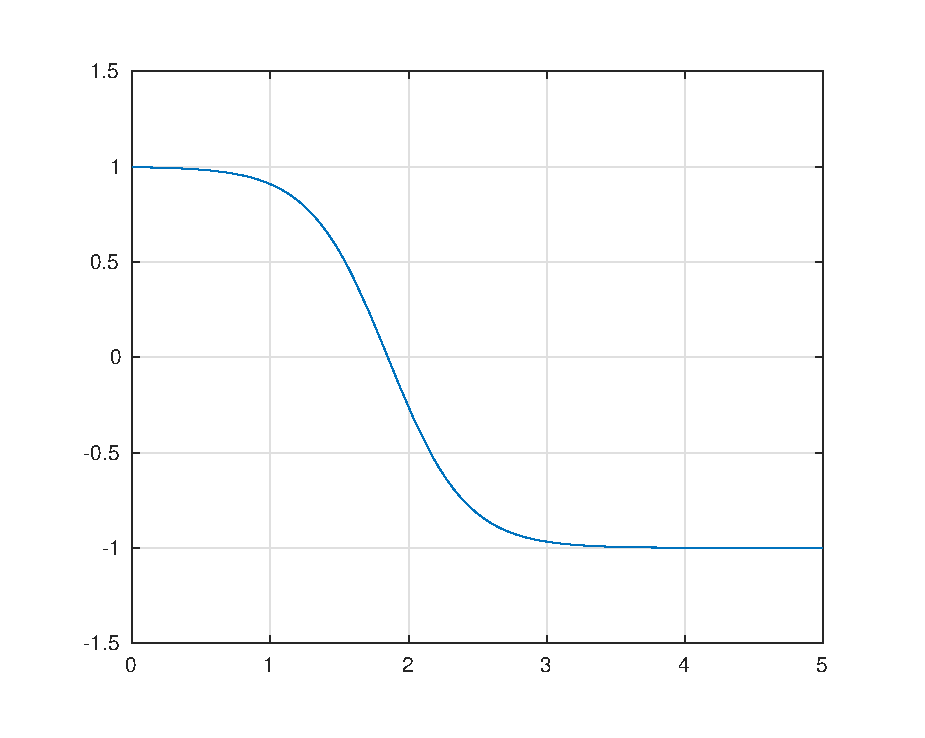
\includegraphics[width=0.4\textwidth]{figures/sig185.eps}
    \caption{Example plot of the CA system's function for adjusting its trust level.}
    \label{fig:sig185}
\end{figure}

\begin{table}[h]
\centering
\begin{tabular}{rlrrrr}
\hline
\textit{} & Category & \#Users & ANGA & ANIA & \#Imp. ND \\ \hline
\multirow{4}{*}{\textit{\begin{tabular}[c]{@{}r@{}}SO 2.0\\ NO 2.3\end{tabular}}} & +/+ & 6 & 139010 & 529 & 0 \\
 & +/- & 2 & 759945 & 4749 & 12 \\
 & -/+ & 24 & 4408 & 932 & 0 \\
 & -/- & 14 & 5110 & 3107 & 33 \\ \cline{2-6} 
 & Summary & 46 & 8973 & 1707 & 45 \\ \hline
\multirow{4}{*}{\textit{\begin{tabular}[c]{@{}r@{}}SO 2.3\\ NO 2.6\end{tabular}}} & +/+ & 5 & 13475 & 283 & 0 \\
 & +/- & 1 & 139525 & 5252 & 7 \\
 & -/+ & 35 & 3022 & 712 & 0 \\
 & -/- & 5 & 4071 & 2090 & 7 \\ \cline{2-6} 
 & Summary & 46 & 7240 & 914 & 14 \\ \hline
\multirow{4}{*}{\textit{\begin{tabular}[c]{@{}r@{}}SO 2.6\\ NO 2.9\end{tabular}}} & +/+ & 3 & 9372 & 251 & 0 \\
 & +/- & 1 & 139525 & 4335 & 5 \\
 & -/+ & 38 & 3041 & 596 & 0 \\
 & -/- & 4 & 3400 & 1499 & 6 \\ \cline{2-6} 
 & Summary & 46 & 6452 & 734 & 11 \\ \hline
\multirow{4}{*}{\textit{\begin{tabular}[c]{@{}r@{}}SO 3.0\\ NO 3.3\end{tabular}}} & +/+ & 3 & 9372 & 234 & 0 \\
 & +/- & 1 & 139525 & 4014 & 4 \\
 & -/+ & 38 & 2671 & 548 & 0 \\
 & -/- & 4 & 3396 & 1389 & 6 \\ \cline{2-6} 
 & Summary & 46 & 6146 & 676 & 10 \\ \hline
\multirow{4}{*}{\textit{\begin{tabular}[c]{@{}r@{}}SO 2.3\\ NO 3.3\end{tabular}}} & +/+ & 3 & 9372 & 249 & 0 \\
 & +/- & 1 & 139525 & 4747 & 7 \\
 & -/+ & 37 & 3064 & 556 & 0 \\
 & -/- & 5 & 3577 & 1646 & 7 \\ \cline{2-6} 
 & Summary & 46 & 6497 & 746 & 14 \\ \hline
\end{tabular}
\caption{CA results achieved by adjusting Single Occurrence (SO) and No Occurrences (NO) parameters.}
\label{tab:adjusting-SO-NO}
\end{table}

\section{Reference cutoff}
\label{sec:analysis-cutoff}
\todo{If we remove this section, remember to remove reference to it in system design chapter.}
\section{Outliers}
\label{sec:analysis-outliers}
\todo{If we remove this section, remember to remove reference to it in system design chapter.}
%SHOW DIFFERENCE BETWEEN USING / NOT USING 20K CUTOFF? ALSO OUTLIERS?
\todo{Mention how we have also tried using personal reward thresholds.}

